\documentclass[a4paper,12pt]{article}
\addtolength{\oddsidemargin}{-1.cm}
\addtolength{\textwidth}{2cm}
\addtolength{\topmargin}{-2cm}
\addtolength{\textheight}{3.5cm}
\newcommand{\HRule}{\rule{\linewidth}{0.5mm}}
\makeindex

\usepackage{longtable}
\usepackage[pdftex]{graphicx}
\usepackage{makeidx}
\usepackage{hyperref}
\usepackage{verbatim}
\hypersetup{
    colorlinks=true,
    linkcolor=blue,
    filecolor=magenta,      
    urlcolor=cyan,
}


% define the title
\author{IMAPKD}
\title{ User Manual}
\begin{document}
\setlength{\parskip}{6pt}

% generates the title
\begin{titlepage}

\begin{center}
% Upper part of the page       

\includegraphics[width=1\textwidth]{./Logo.png}\\[0.4cm]

%Title

\HRule \\[0.4cm]
{ \huge \bfseries User Manual}\\[0.1cm]
\HRule \\[0.4cm]  

% Group Members 

\begin{minipage}{0.4\textwidth}
\begin{flushleft} \large

\emph{\Large Group Members:}\\[0.4cm]    
\emph{}\\
{\Large Diana {Obo}} \\
\emph{}\\
\emph{}\\
{\Large Priscilla {Madigoe}}\\
\emph{}\\
\emph{}\\
{\Large Kudzai {Muranga}} \\
\emph{}\\
\emph{}\\
{\Large Sandile {Khumalo}}\\
\emph{}\\
\emph{}\\

\end{flushleft}
\end{minipage}
\begin{minipage}{0.4\textwidth}
\begin{flushright} \large

\emph{ \Large Student numbers:} \\[0.4cm]  
\emph{}\\
{\Large u13134885}\\
\emph{}\\
\emph{}\\
{\Large u13049128}\\
\emph{}\\
\emph{}\\
{\Large u13278012}\\
\emph{}\\
\emph{}\\
{\Large u12031748}\\
\emph{}\\
\emph{}\\

\end{flushright}
\end{minipage}

% bottom section of title page

{\large \today}
\end{center}
\end{titlepage}
\renewcommand{\thesection}{\arabic{section}}

\newpage
\begin{center}
\textsc{\Large Client}\\[0.5cm]
CSIR - Council for Scientific and Industrial Research\\[0.5cm]
\textsc{\Large IMPAKD link}\\[0.5cm]
For further references see \href{https://github.com/u13278012/IMPAKD/}{gitHub}.
\today
\end{center}
\newpage
\tableofcontents{}

\newpage 
\section{Introduction}
This document is a user manual for a Property Investment Optimizer web application. It was developed by team IMPAKD for CSIR at the University of Pretoria (2016).The code is available as open source on \href{https://github.com/u13278012/IMPAKD/}{gitHub}. Below is a walk through of the installation and guidelines on how to use the application. Advanced users who are familiar with coding are more than welcome to use their own way of installation. 

\section{Vision}
The Property Investment Optimizer application's objective is to evaluate whether a certain rental property is worth buying. It does this by calculating the Return of Investment (ROI) of a property, which can be compared with another property's ROI, to assist a user to optimize their investment strategy according to their portfolio.\\\\
The project will assist the user by helping to answer the following questions:\begin{itemize}
	\item Given a certain bond (interest rate, deposit as a percentage of property value), rental (occupancy rate, agent commission, rental amount) and environmental conditions (Interest rate, inflation) what is the ROI?
	\item When is it better to pay a higher or lower deposit for a bond?
	\item Between two rental scenarios which provides the greater ROI?
	\item Is it better to try and pay off the bond as fast as possible by paying in extra capital?
	\item How does purchasing another property influence a user's ROI and at which point would this be a good idea?
	\item At which point does it make sense to buy another property?
	\item How much tax will the user have to pay?s

\end{itemize}

\section{Background}
The project was given to us by our client, CSIR, so that we can research how the ROI of different configurations of rental properties can answer the questions listed in the Vision section of this document. Answers to these questions can be used to help users of the system choose to buy the best property that fits their portfolio and requirements with the ease of not having to manually evaluate the property themselves. The project can also be used for property-related research.


\section{System Overview}

The Property Investment Optimizer application is designed to assist the user to know when is the right time to buy property and when is the right time to sell property. It also tells the user the best option to pay off a bond, which is either higher or lower. A user is allowed to add a property to calculate the property's ROI which is then added to the user's portfolio. Two properties can be compared to see which one has a better return of investment. Furthermore, the application will simulate the buying of properties. This application contains basic functionality, which is easy to use. The project is split into the back-end server and the front-end website.
\section{System Configuration}
A Windows/Unix based host  is required to run the application's back end server. This
host must have the associated technologies installed (the installation of these
technologies is illustrated below). The host must have internet connectivity in order to allow any of the required dependencies to be installed and set
up for the operating system environment. The back-end server runs on port 8080 and the website runs on port 8383.



The system uses REST web services to send data between the back-end server and the website. The data from the back-end server is sent in xml format and is translated to json objects on the website. From the website, the data is sent as encodedString and application-form-urlencoded media types using Ajax calls.The systems data is stored on a PostgreSQL database.

Users of the website will only be required to have a device that has a web browser and access to the internet.

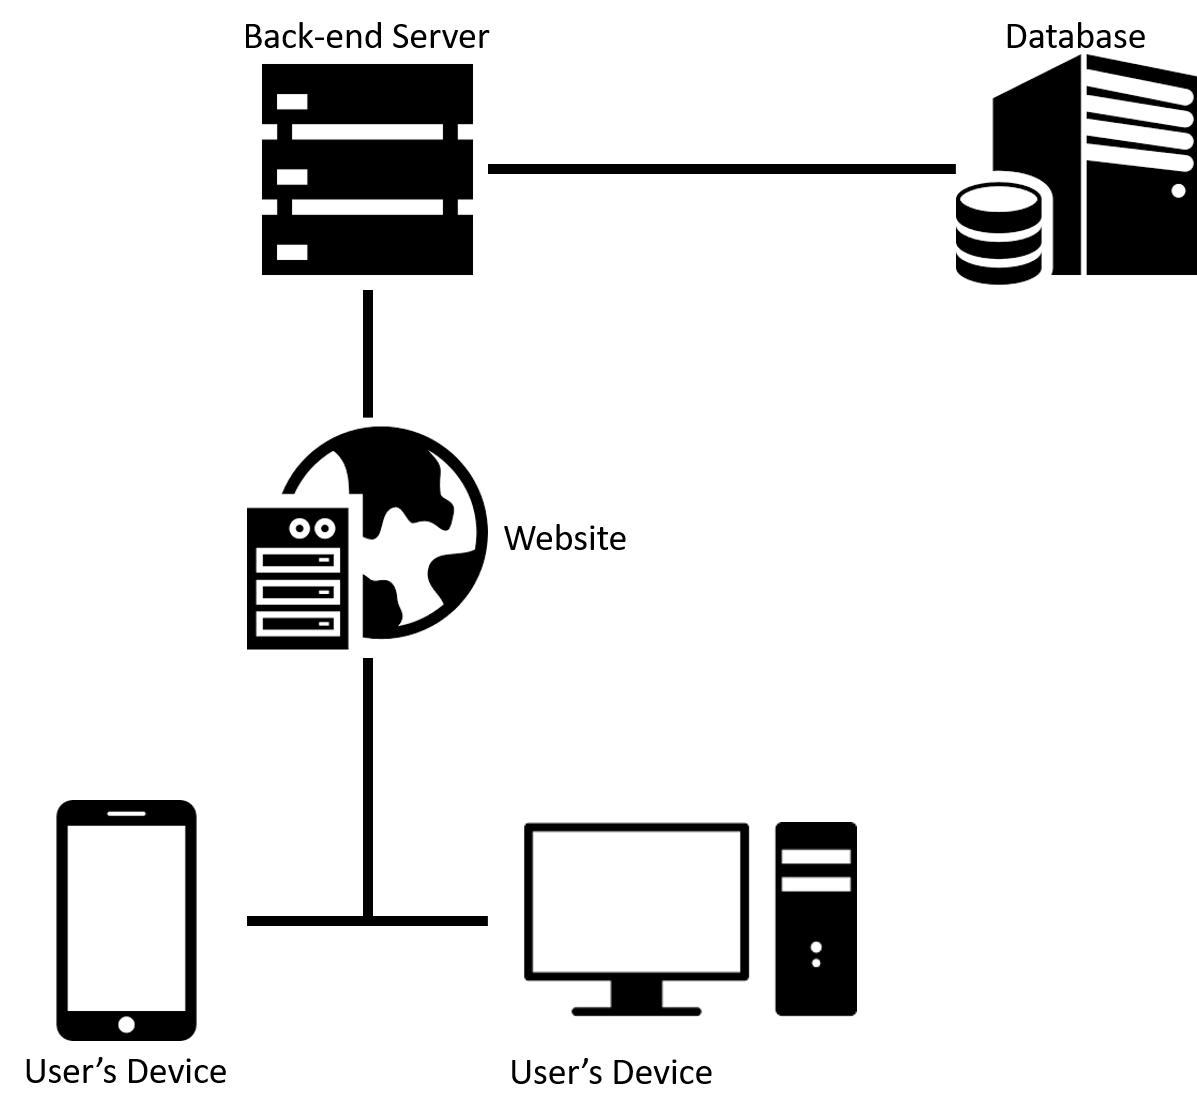
\includegraphics[width=0.9\linewidth, center]{./System/system.png}\\[0.4cm]

\section{Installation}

\subsection{Prerequisites}
In order to use the Property Investment Optimizer system, you must install the following the technologies:
\begin{itemize}
\item{AngularJS - \href{https://angularjs.org/}{link}}
\item{Apache Maven - \href{https://maven.apache.org/download.cgi}{link}}
\item{Glassfish Server - \href{https://glassfish.java.net/download.html}{link}}
\item{Java JDK - \href{http://www.oracle.com/technetwork/java/javase/downloads/index.html}{link}}
\item{Netbeans - \href{https://netbeans.org/downloads/}{link}}
\item{Node.js - \href{https://nodejs.org/en/download/}{link}}
\item{PostgreSQL - \href{https://www.postgresql.org/download/}{link}}
\end{itemize}
You must first download the project from the following link: \href{https://github.com/u13278012/IMPAKD}{Github}. After you have downloaded the project, follow the instructions below to install the required technology.


\newpage
\subsubsection{Installing Apache Maven}
\begin{enumerate}
\item Go to the following link: \href{https://maven.apache.org/download.cgi}{apacheMaven link}\\[0.2cm]
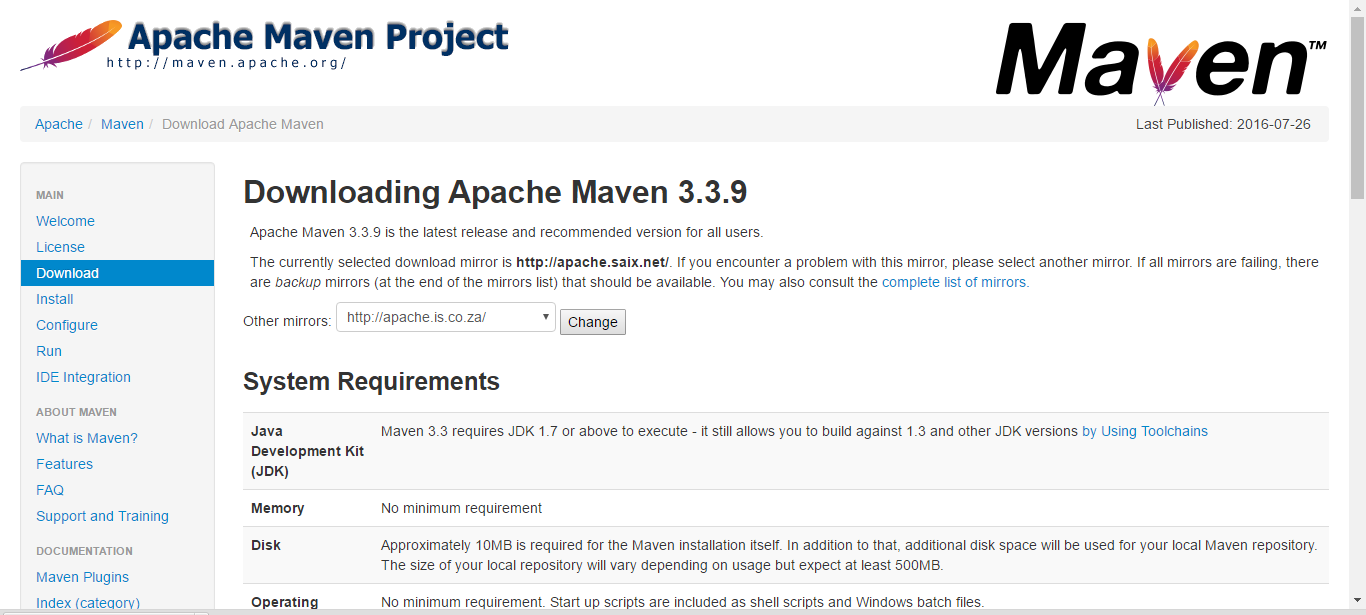
\includegraphics[width=0.9\linewidth, center]{./Installation/maven_download_1.PNG}\\[0.4cm] 
 
\item Click your preferred download link under the the 'Files' Section of the page\\[0.2cm]

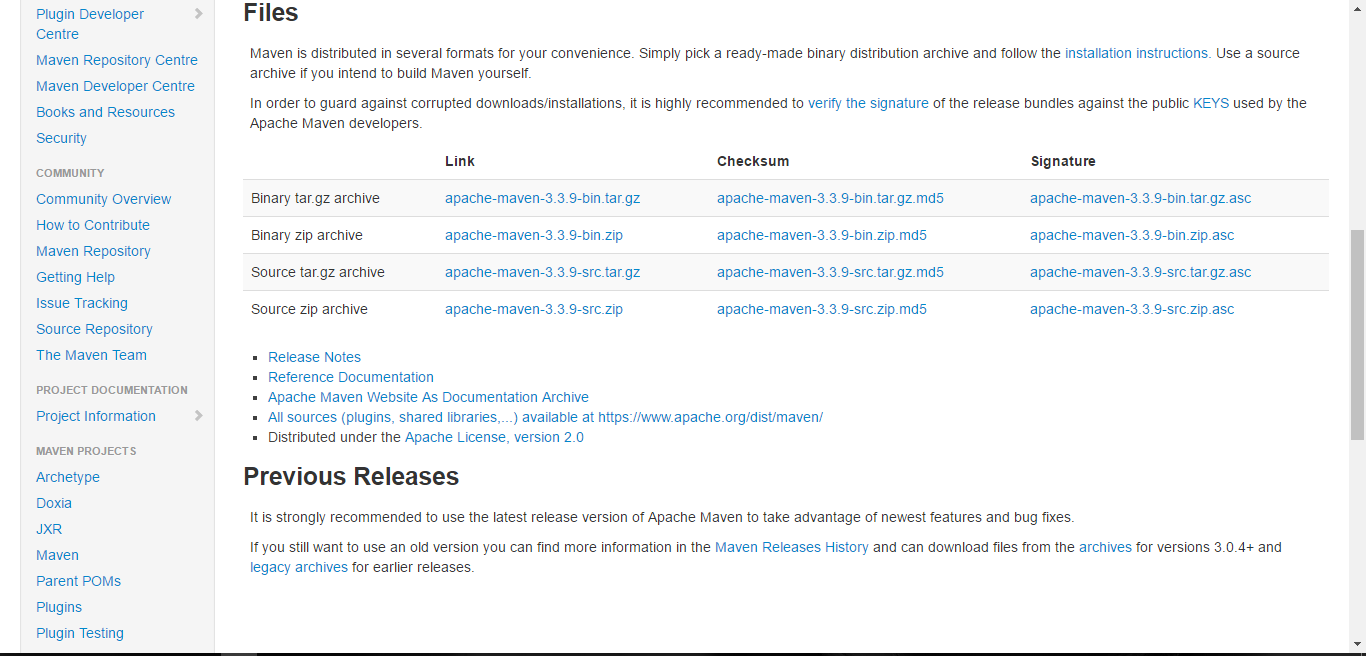
\includegraphics[width=0.9\linewidth, center]{./Installation/maven_download_2.PNG}\\[0.4cm] 

\newpage
\item Open the command prompt by pressing the windows key together with the letter 'r', win+R, and type 'cmd'.

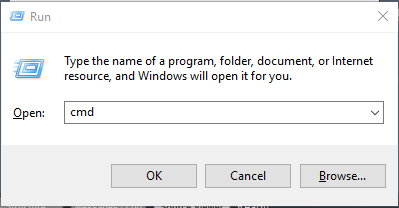
\includegraphics[width=0.9\linewidth, center]{./Installation/maven_download_3.PNG}\\[0.4cm] 
 
\item Once open, type the following command: unzip Apache-maven-3.3.9-bin.zip, in the folder that contains the download, to extract the data.
\item Open the Control Panel.

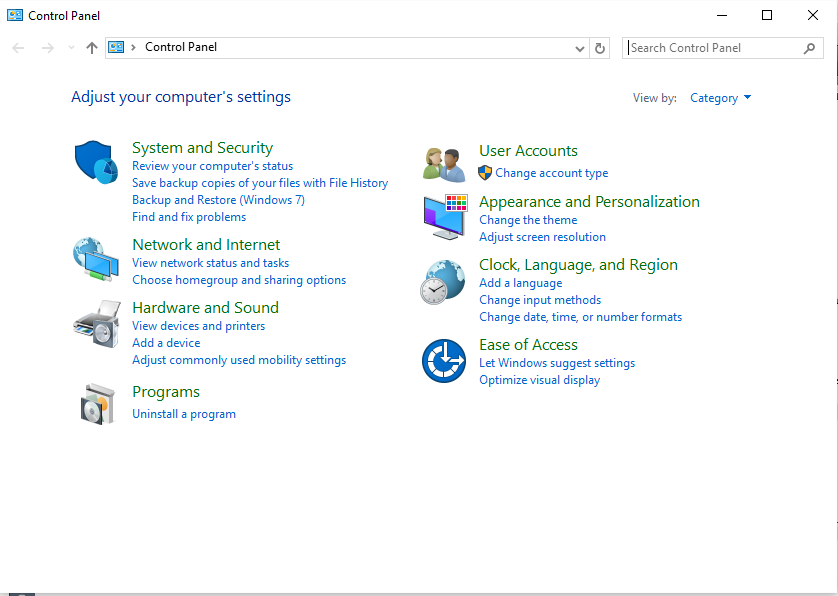
\includegraphics[width=0.9\linewidth, center]{./Installation/maven_download_4.PNG}\\[0.4cm]

\newpage
\item Select System and Security.
\item Select System.
\item Select Advanced System Settings
\item Click the Environment Variable.. button
\item Select the New button under User Variables

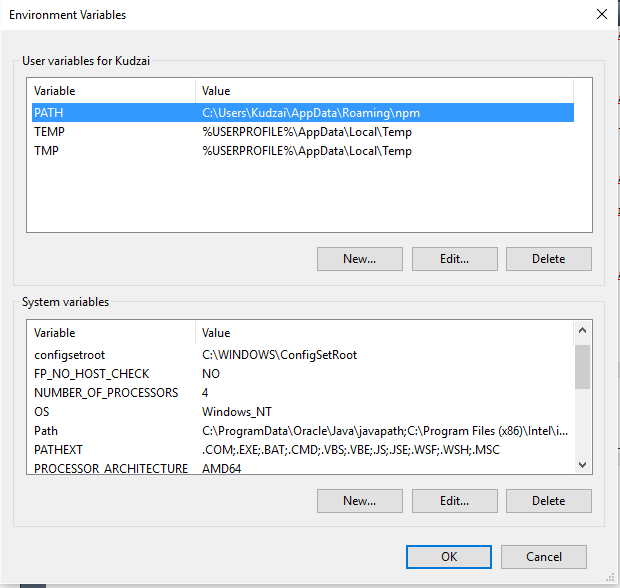
\includegraphics[width=0.9\linewidth, center]{./Installation/maven_download_5.PNG}\\[0.4cm]

\item Add the file directory path of the 'bin' folder for Apache Maven and click OK.
\end{enumerate}

\newpage
\subsubsection{Installing Glassfish Server}
\begin{enumerate}
\item Go to the following link: \href{https://glassfish.java.net/download.html}{glassfishServer link}\\[0.2cm]
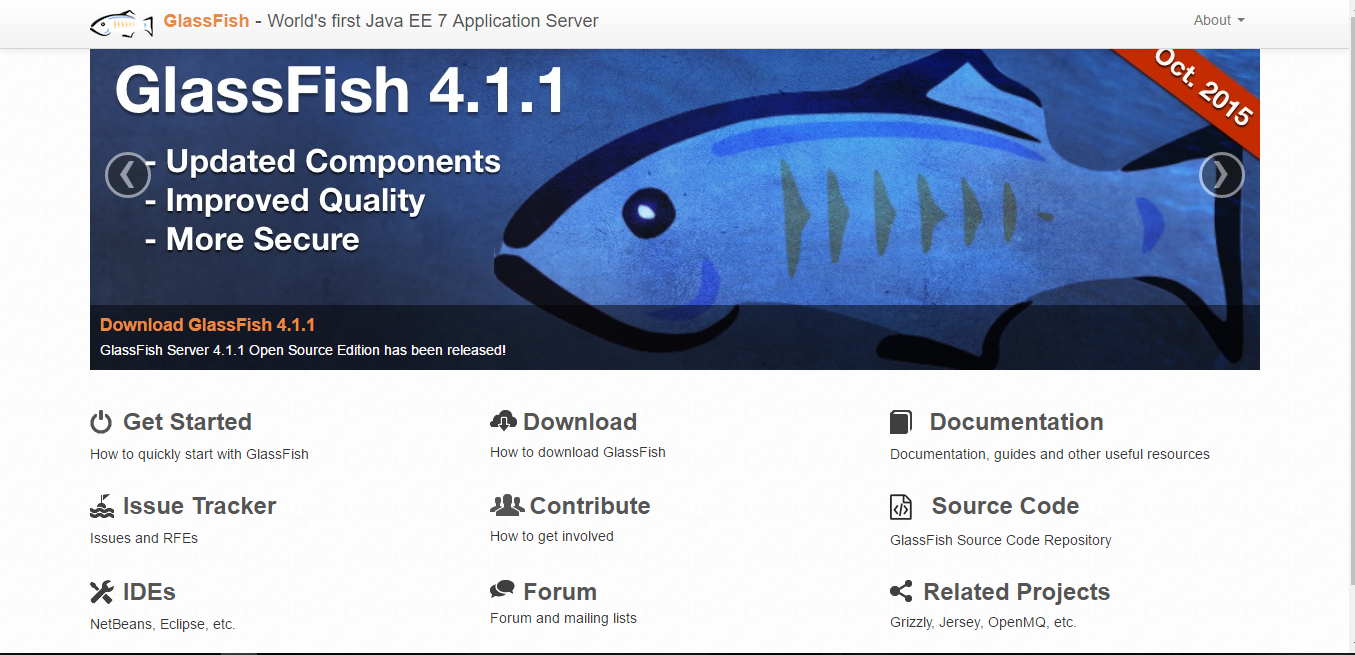
\includegraphics[width=0.9\linewidth, center]{./Installation/glassfish_download_1.PNG}\\[0.4cm]
\item Click the Download link

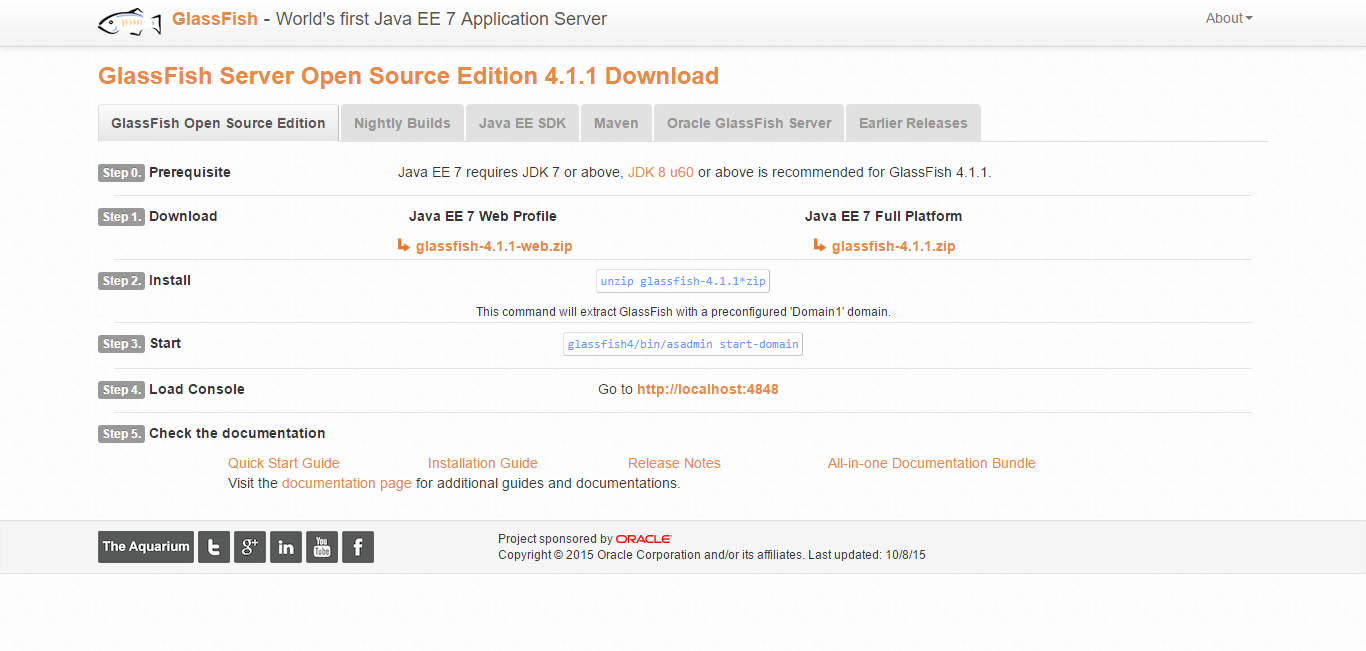
\includegraphics[width=0.9\linewidth, center]{./Installation/glassfish_download_2.PNG}\\[0.4cm]

\item Download  the 'Java EE 7 Full Platform' link and follow the instructions on the page.
\end{enumerate}

\newpage
\subsubsection{Installing Java JDK}
\begin{enumerate}
\item  Go to the following link: \href{http://www.oracle.com/technetwork/java/javase/downloads/index.html}{javaJDK link}

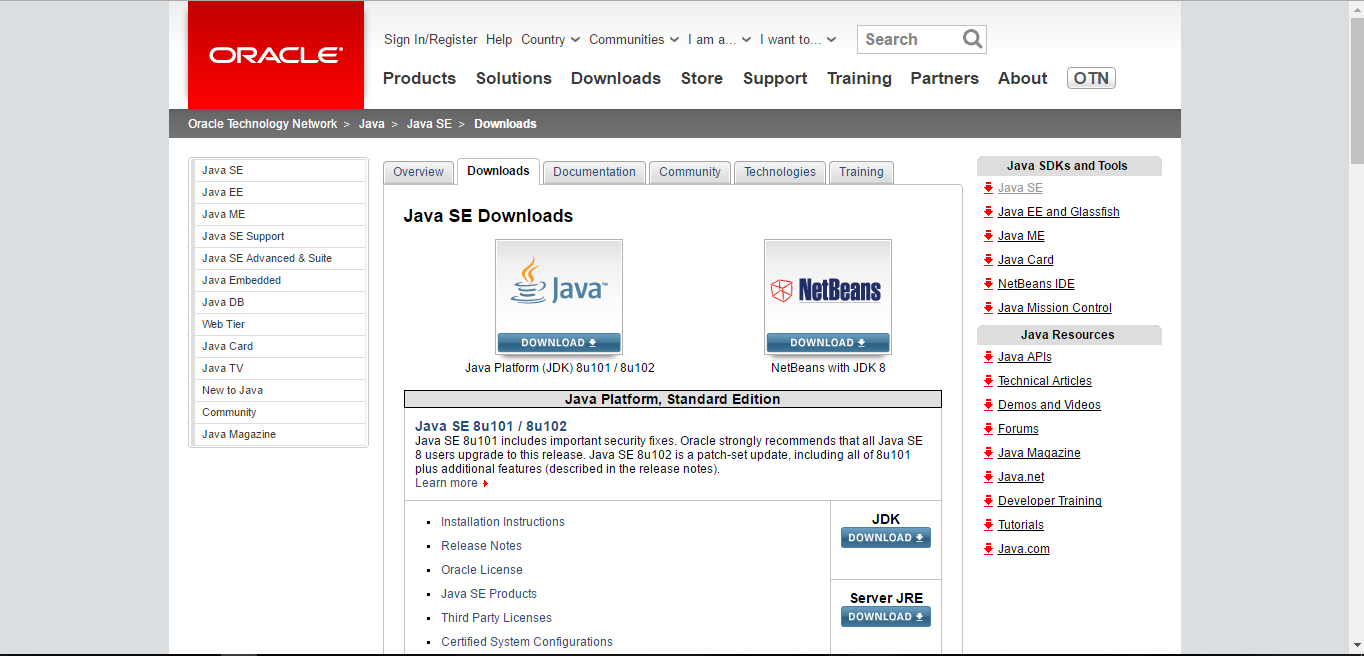
\includegraphics[width=0.9\linewidth, center]{./Installation/Java_download_1.PNG}\\[0.4cm]

\item Click on the 'Java Platform (JDK) 8u101 / 8u102' link.

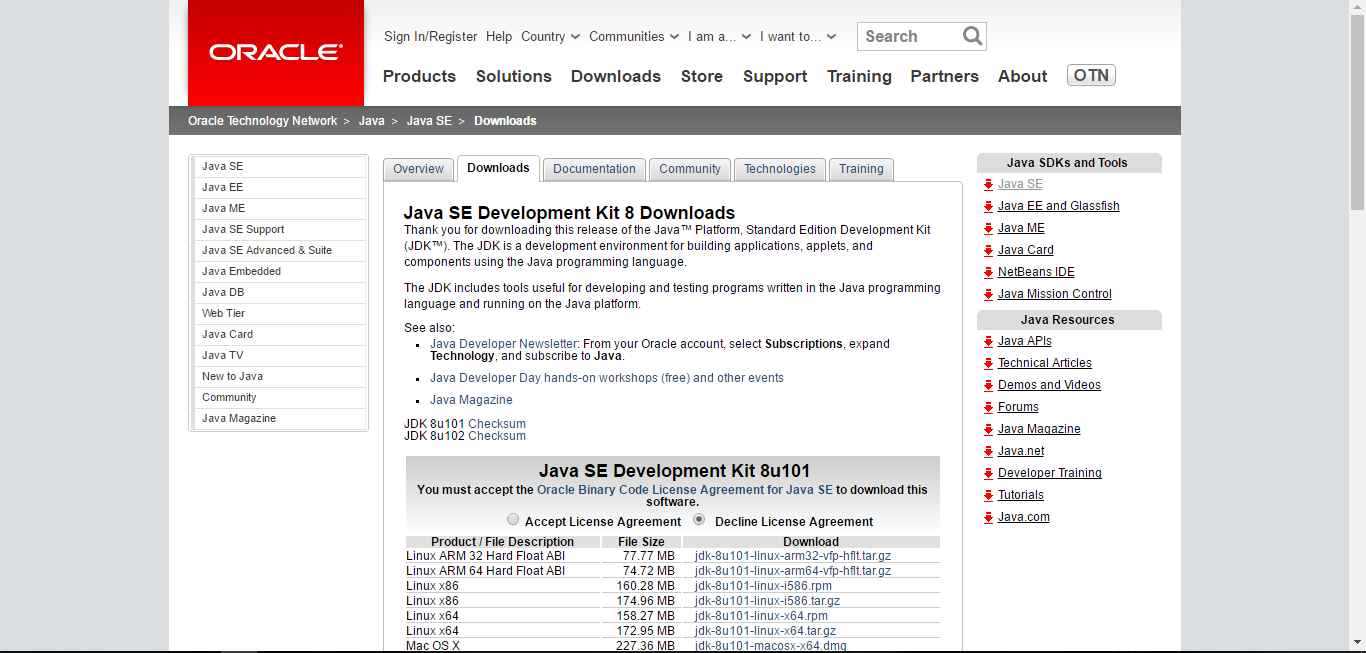
\includegraphics[width=0.9\linewidth, center]{./Installation/Java_download_2.PNG}\\[0.4cm]

\item Select your required version and download it.
\item Once downloaded, open the installation file and follow the prompts to install it.
\end{enumerate}

\newpage
\subsubsection{Installing Netbeans}
\begin{enumerate}
\item Go to the following link: \href{https://netbeans.org/downloads}{Netbeans link}\\[0.2cm]
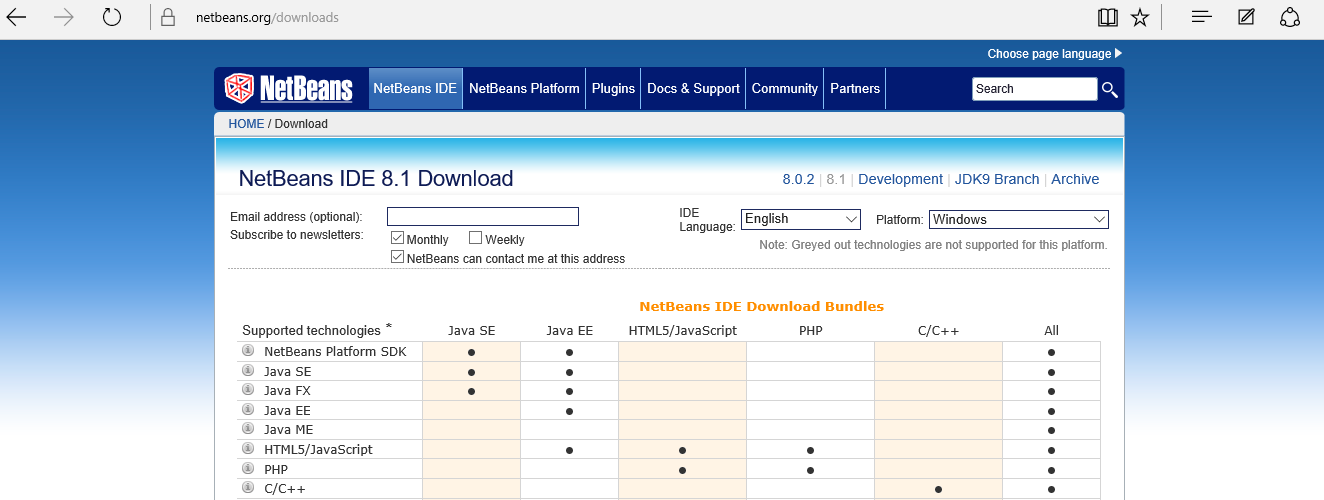
\includegraphics[width=0.9\linewidth, center]{./Installation/mavenlink.PNG}\\[0.4cm] 
 
\item download this version\\\\
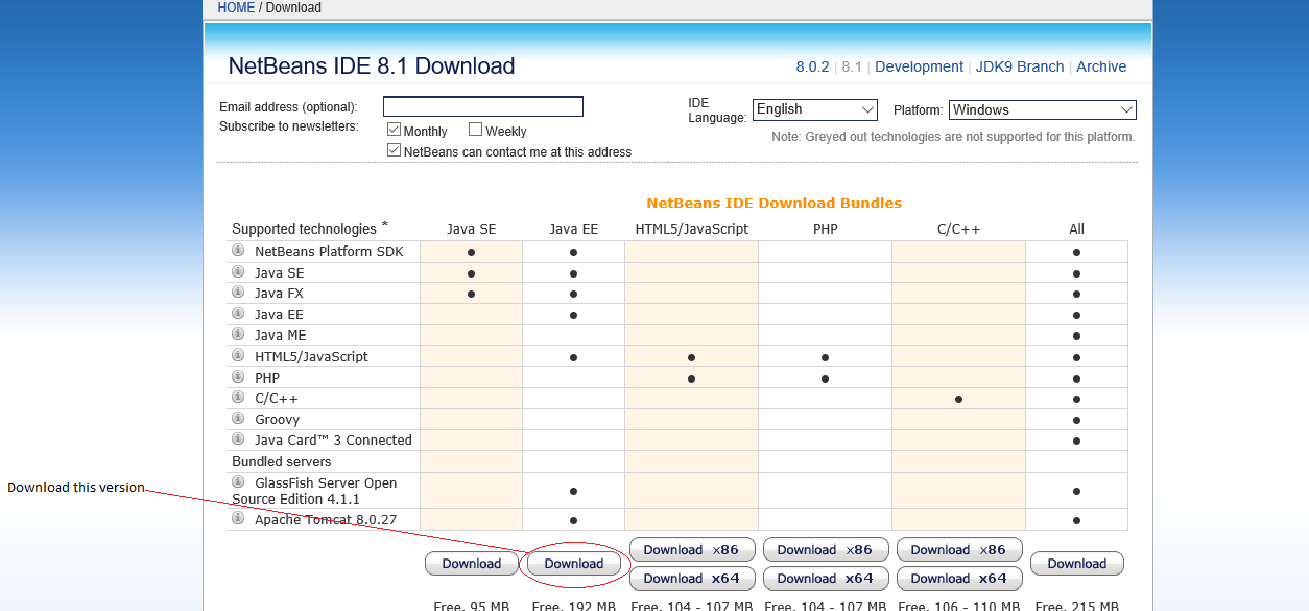
\includegraphics[width=0.9\linewidth, center]{./Installation/maven.PNG}\\[0.4cm] 
 
\item run the downloaded .exe file and follow the prompts to install it\\
\end{enumerate}
\subsubsection{Installing Node.js}

\begin{enumerate}
\item Go to the following link: \href{https://nodejs.org/en/}{Node.js link}\\[0.2cm]
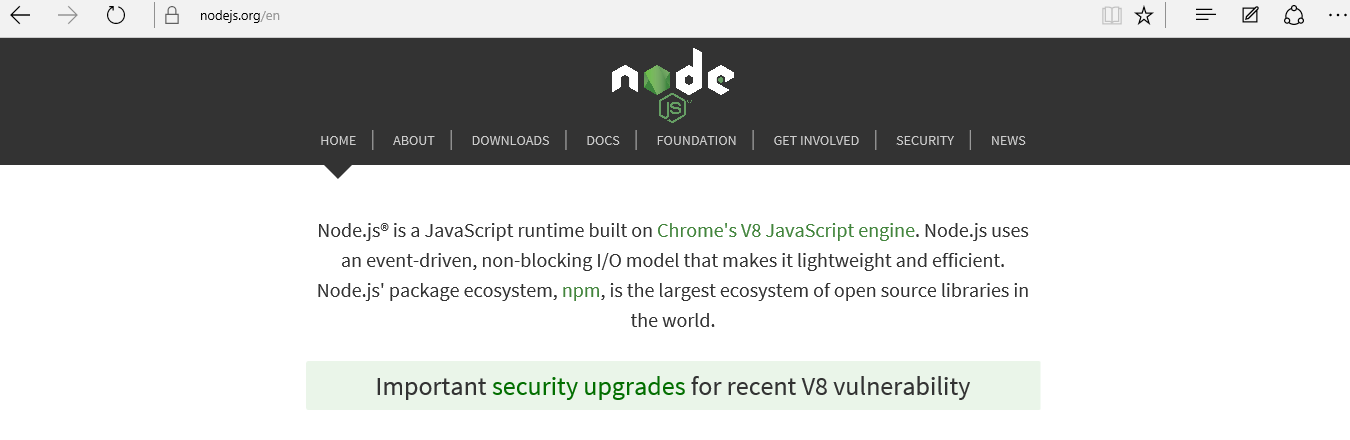
\includegraphics[width=0.9\linewidth, center]{./Installation/nodejs_website.PNG}\\[0.4cm] 
 
\item download the desired version preferably the recommended one. See picture below \\
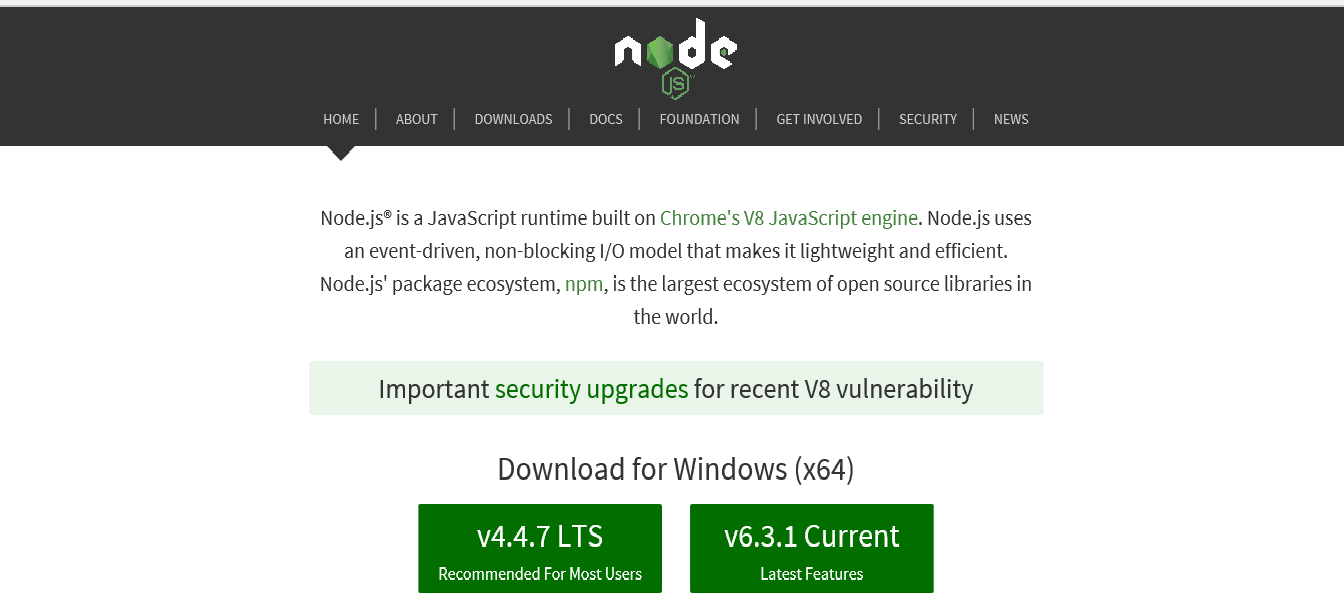
\includegraphics[width=0.9\linewidth, center]{./Installation/nodejs.PNG}\\[0.4cm] 
 
\item run the downloaded .exe file and follow the prompts to install it\\
\end{enumerate}

\subsubsection{Installing PostgreSQL}
\begin{enumerate}
\item You need to download the installer from PostgreSQL Official website.
\item Go to the PostgreSQL official website, download section for Windows\\
\href{http://www.postgresql.org/download/windows/}{PostgreSQL Link}.
\item Click on the download installer from EnterpriseDB
\item Choose the latest version to download. It takes few minutes to complete the download.
\item Double click the installer\\
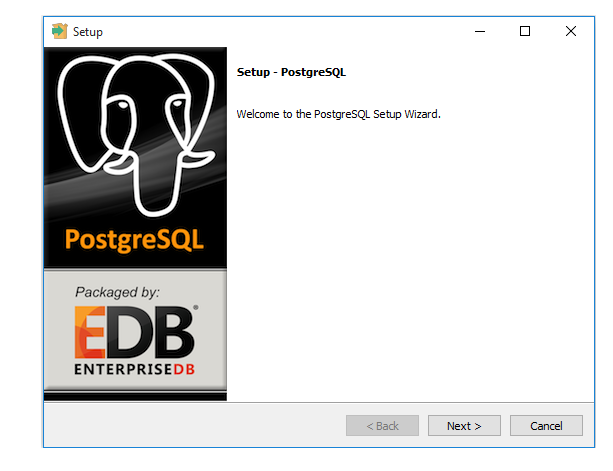
\includegraphics[width=0.9\linewidth, center]{./Installation/postGresql1.PNG}\\[0.4cm]
\item Enter the password for the database superuser and service account. \\ 
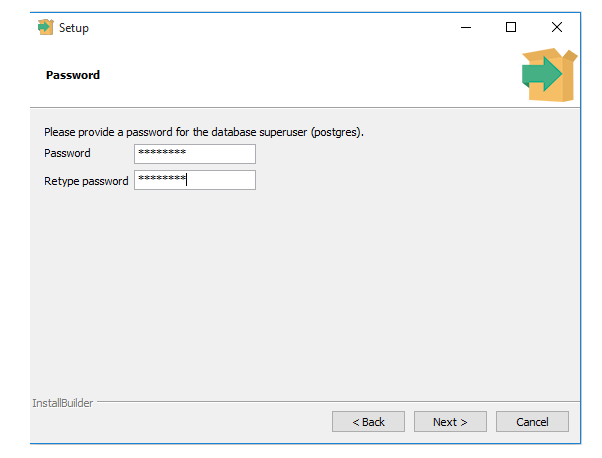
\includegraphics[width=0.9\linewidth, center]{./Installation/postGresql2.PNG}\\[0.4cm]
\newpage
\item Enter the port for PostgreSQL. Make sure that no other applications are using this port. Leave it as default if you are unsure \\ 
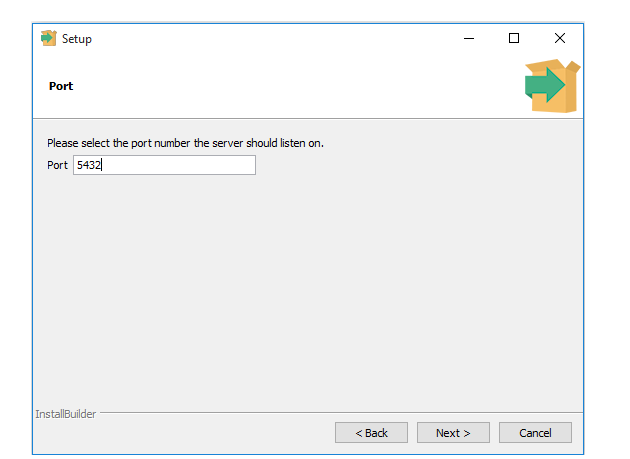
\includegraphics[width=0.9\linewidth, center]{./Installation/postGresql3.PNG}\\[0.4cm]
\item Choose the default locale used by the database. \\ 
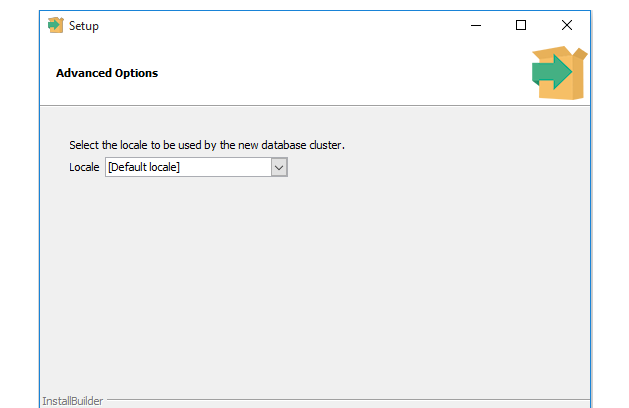
\includegraphics[width=0.9\linewidth, center]{./Installation/postGresql4.PNG}\\[0.4cm]
\newpage
\item Wait for it to finish installing \\ 
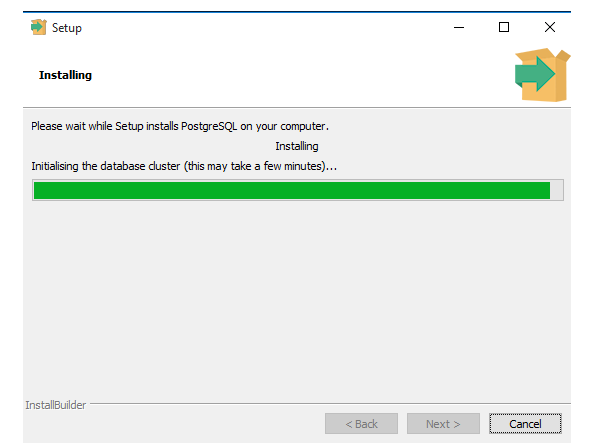
\includegraphics[width=0.9\linewidth, center]{./Installation/postGresql5.PNG}\\[0.4cm] 
\item Click finish \\
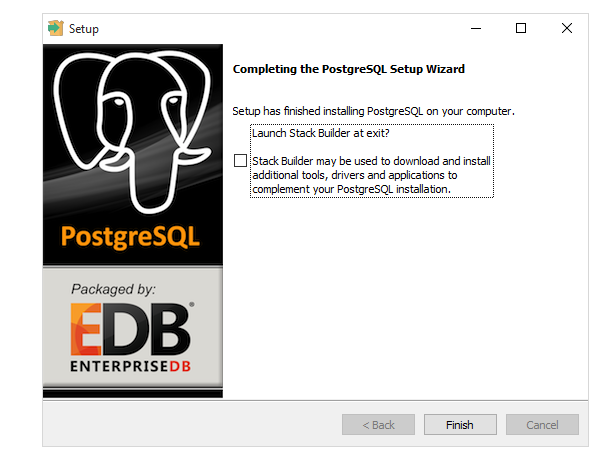
\includegraphics[width=0.9\linewidth, center]{./Installation/postGresql6.PNG}\\[0.4cm] 

\end{enumerate}

\subsection{Setting up the System}
Open Netbeans and open the 'BackEndPIO' netbeans project from the project folder. Once opened, run the project in order to start the Glassfish serve. BackEndPIO runs on port 8080.\\
Once 'BackEndPIO' is running, open the 'FrontEnd' netbeans project from the project folder. Once opened, run the project. 'FrontEnd' runs on port 8383.

\section{Using The System}
%Home Page
\subsection{Home Page}
		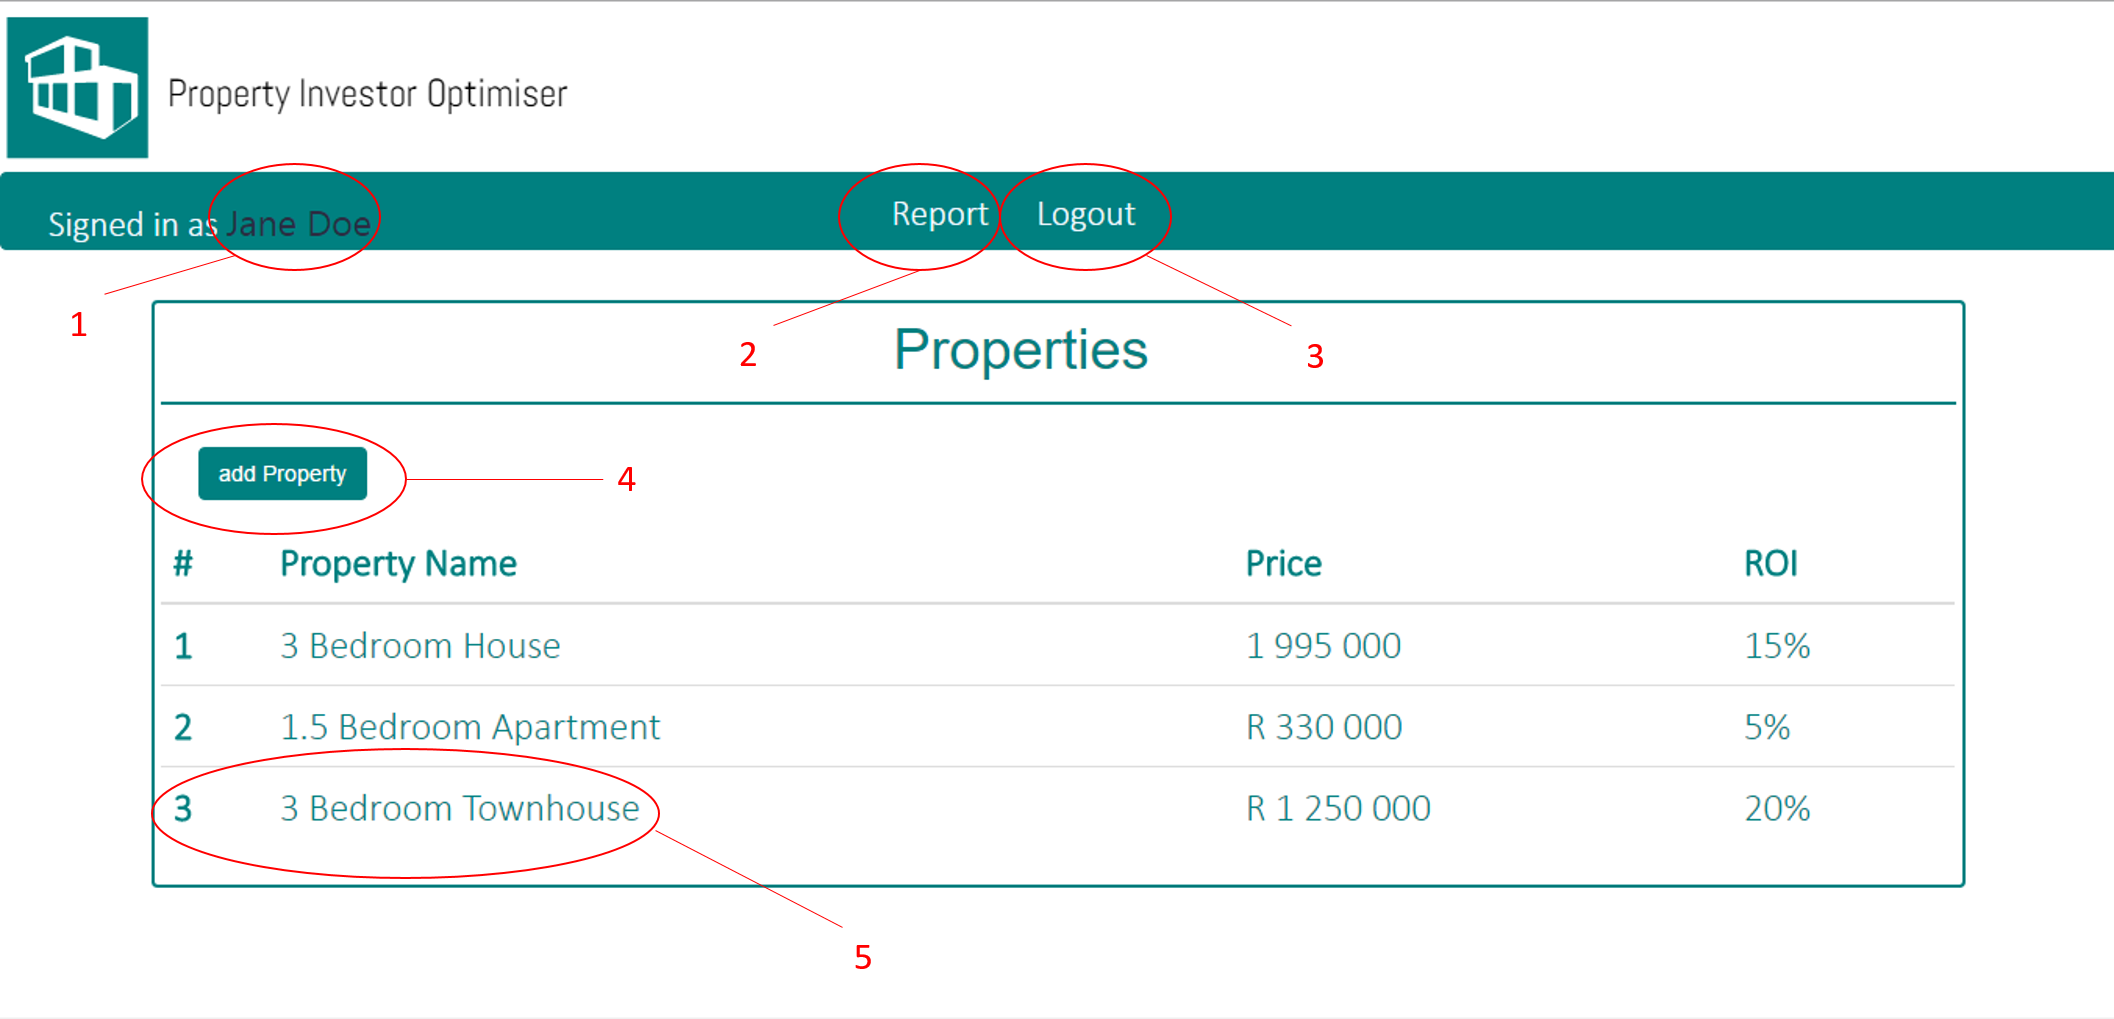
\includegraphics[width=0.9\linewidth, center]{./System/Home.PNG}\\[0.4cm]  
Once the user has successfully logged into the system, the user will see this page. This page facilitates the following functionalities:
	\begin{enumerate}
		\item{\underline{\bfseries Profile}}\\[0.2cm] 
		When the user clicks their name, the system will navigate to the profile page that will display their personal details. 				The user can change his/her details accordingly. They will also be able to see the number of properties associated 				with their profile.
		\bigskip
		\item{\underline{\bfseries Report}}\\[0.2cm] 
		This functionality will enable the user to generate a report about certain properties in a pdf file. Based on several calculations 				configured for certain properties, the report will contain the calculation results and display the Return of Interest based 			on the calculations. 
		\bigskip
		\item{\underline{\bfseries Logout}}\\[0.2cm] 
		This button will log the user out of the system. Once this option has been selected, the user will not be able to use the 				system. They will be redirected to the "main page" where they will need to log in again should they want to use the system 				again. 
		\bigskip
		\item{\underline{\bfseries Add Property}}\\[0.2cm] 
		This button will enable the user to add more details about a certain property. This information will be persisted and 				certain values will be calculated by the system dynamically as the user adds a certain property.
		\bigskip
		\item{\underline{\bfseries View Property Details}}\\[0.2cm] 
		When the user clicks on one of the entries on the table, he/she will be redirected to a page that shows more information 		about the property they have selected.
		\bigskip
		\item{\underline{\bfseries Delete Property}}\\[0.2cm] 
		This button will delete the relevant property from the database. The page will reload and show the updated list.
		\bigskip
		\item{\underline{\bfseries Update Property Details}}\\[0.2cm] 
		This button will allow the user to change the details for a property that has already been added to the list.
	\end{enumerate}

%Add Property
\subsection{Add Property}
		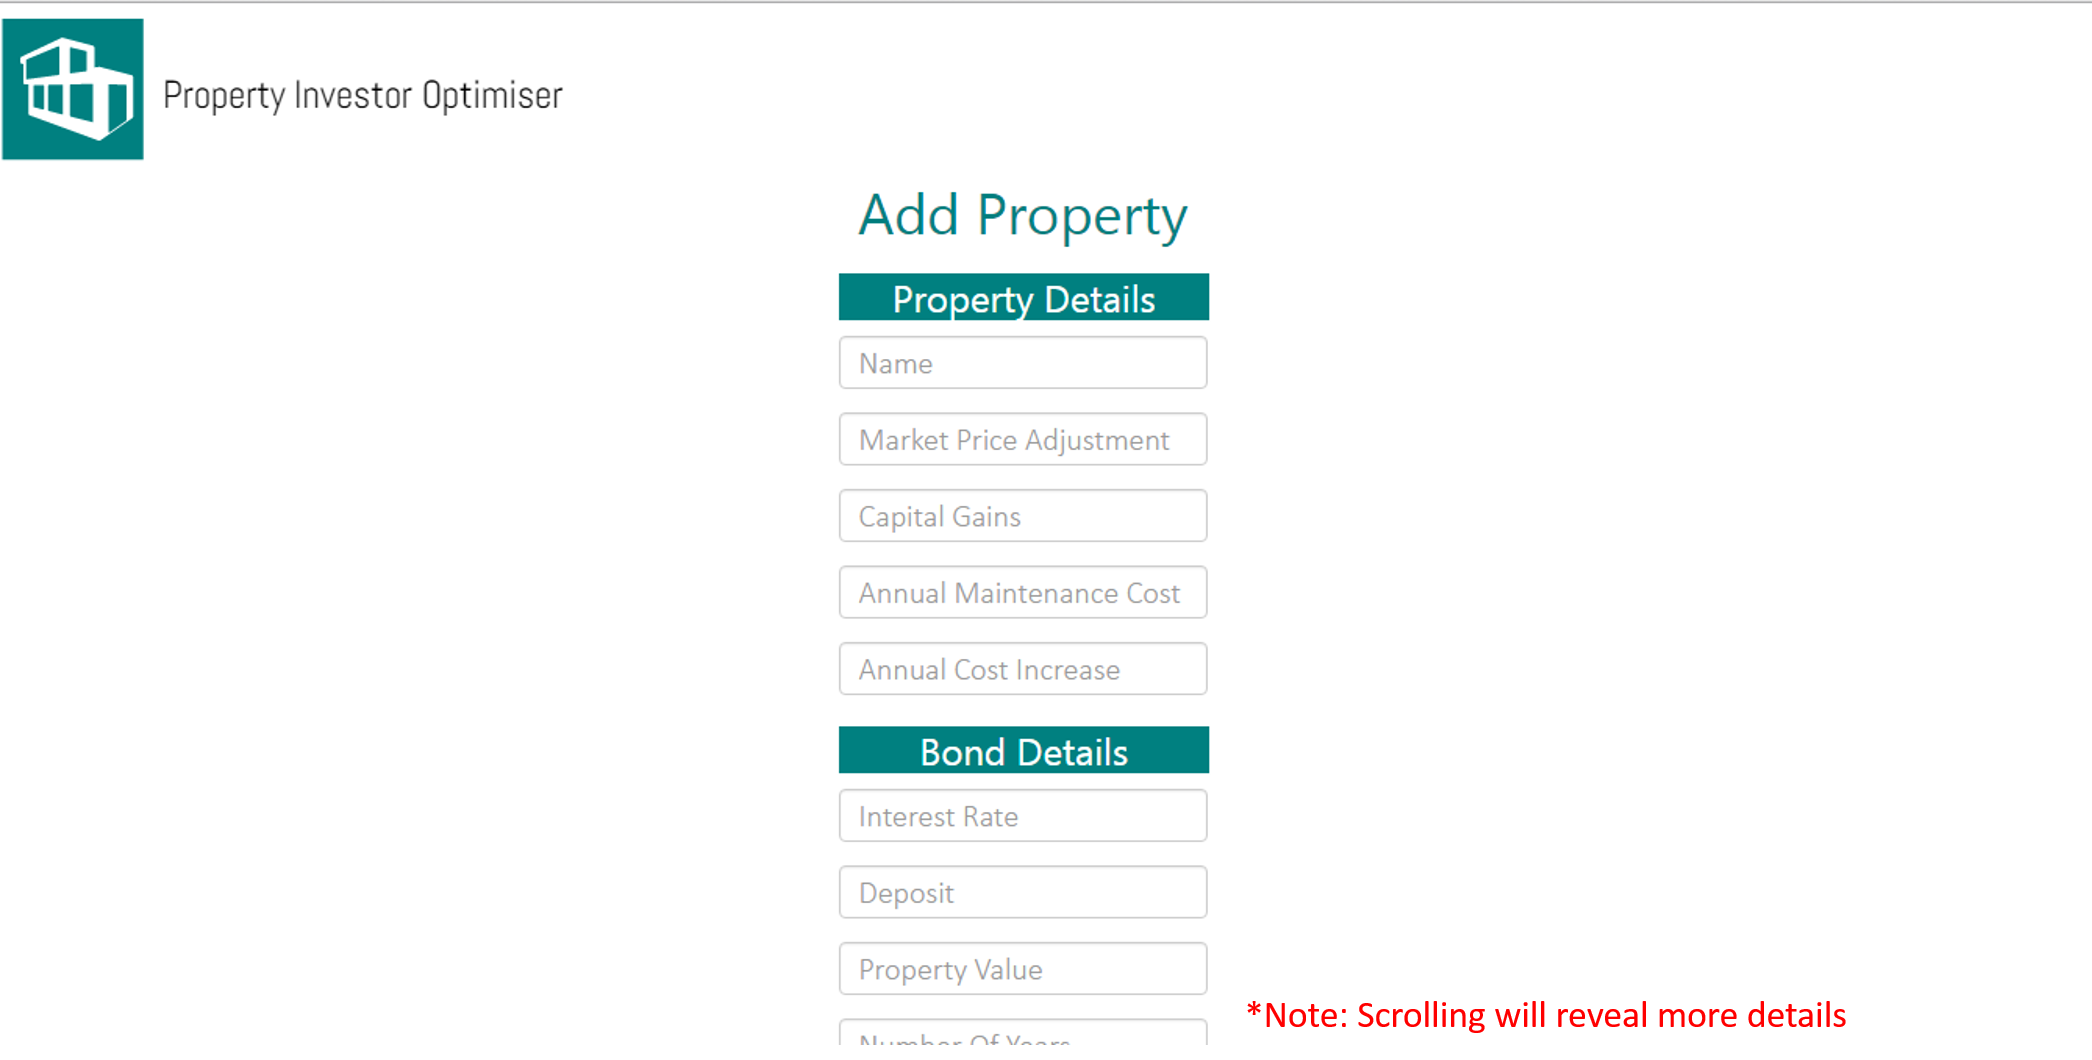
\includegraphics[width=0.9\linewidth, center]{./System/AddProperty.PNG}\\[0.4cm]  
		\caption{Add Property}
As previously mentioned on the fifth point under the "home page" section, this page will enable the user to add a property to the system. Once validated, the details will then be added onto the system. The user needs to add a certain property once. Certain property details can be edited.  

%Property Details
\subsection{Property Details}
		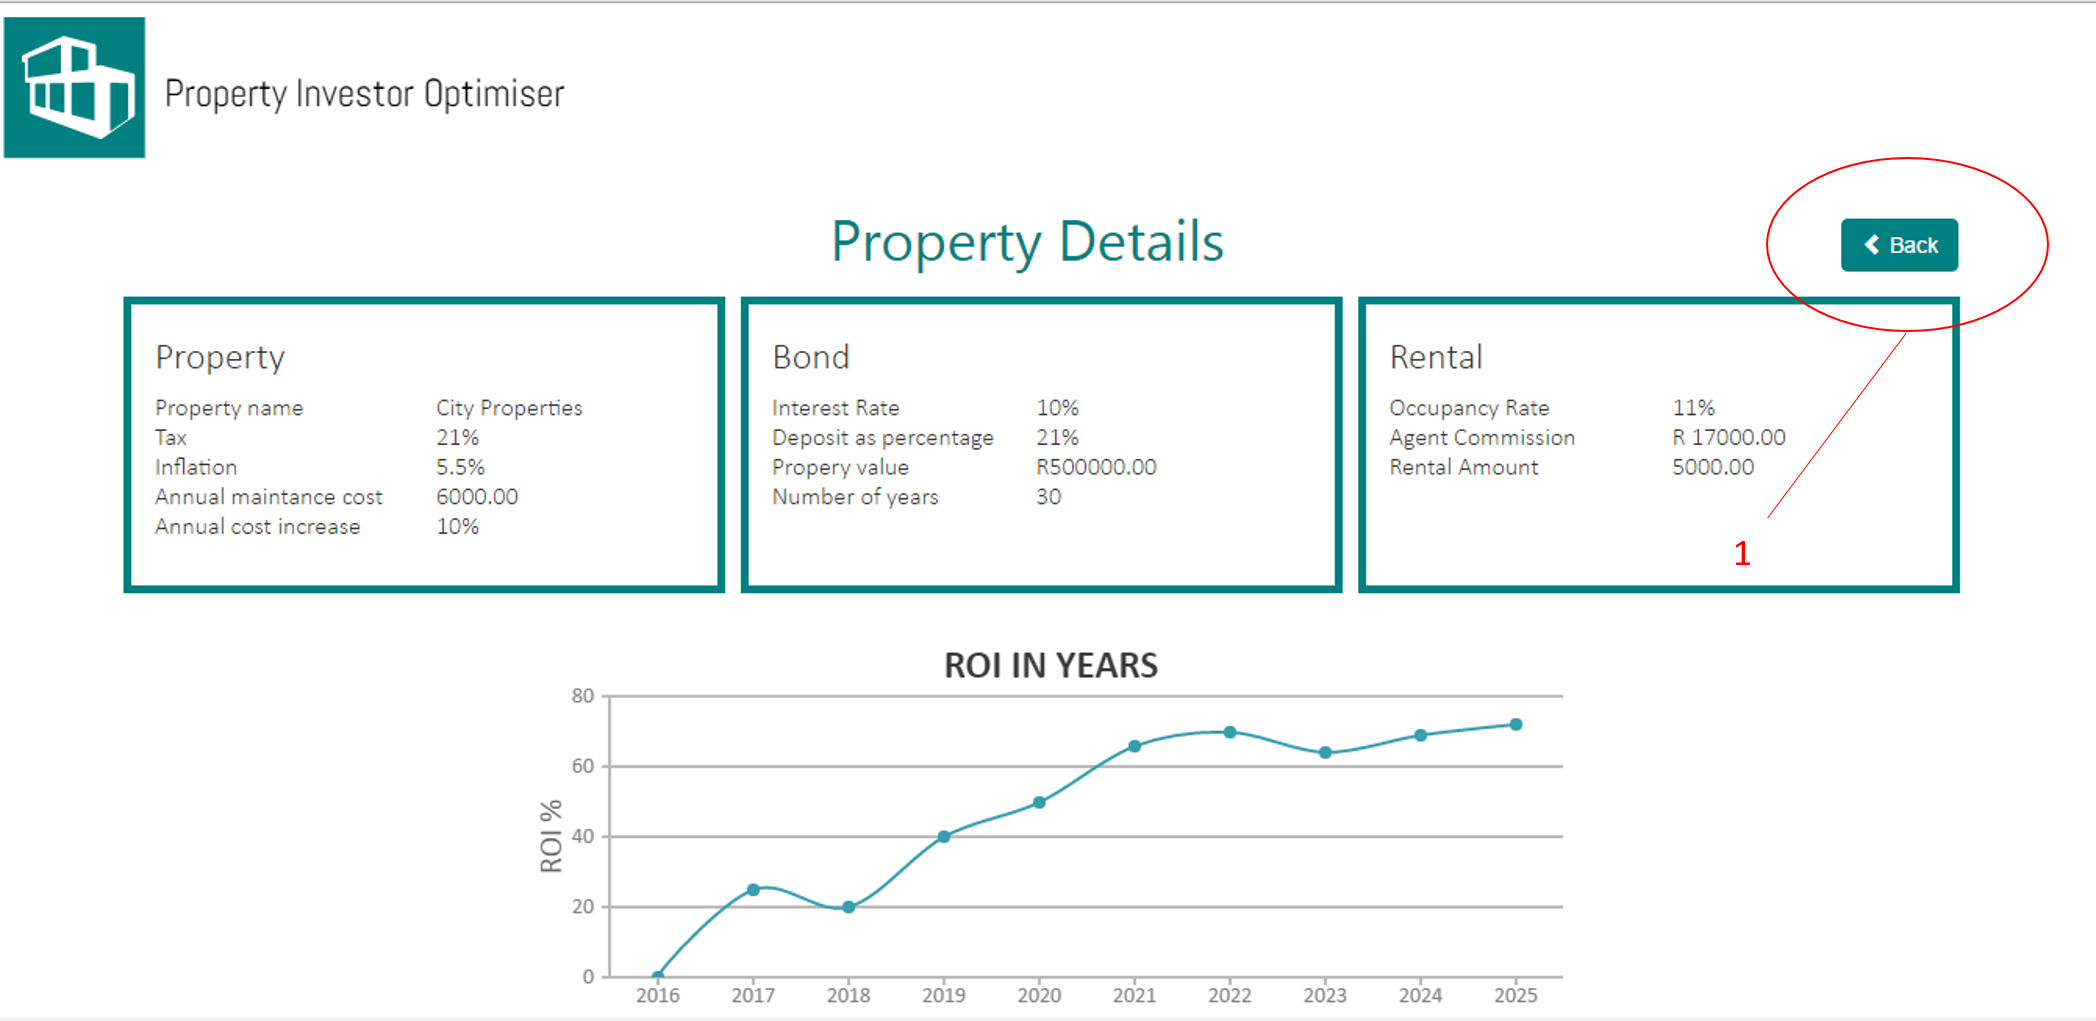
\includegraphics[width=0.9\linewidth, center]{./System/PropertyDetails.PNG}\\[0.4cm]  
		\caption{Property Details}
	As previously mentioned on the fifth point under the "home page" section, this page will enable the user see more details 			about the property they have selected on the "home page". The "ROI In Years" graph will be generated and more information 			pertaining to the property will be displayed.  
	\begin{enumerate}
		\item This button will enable the user to get back to the "home page".
	\end{enumerate}
	
\subsection{Profile}
		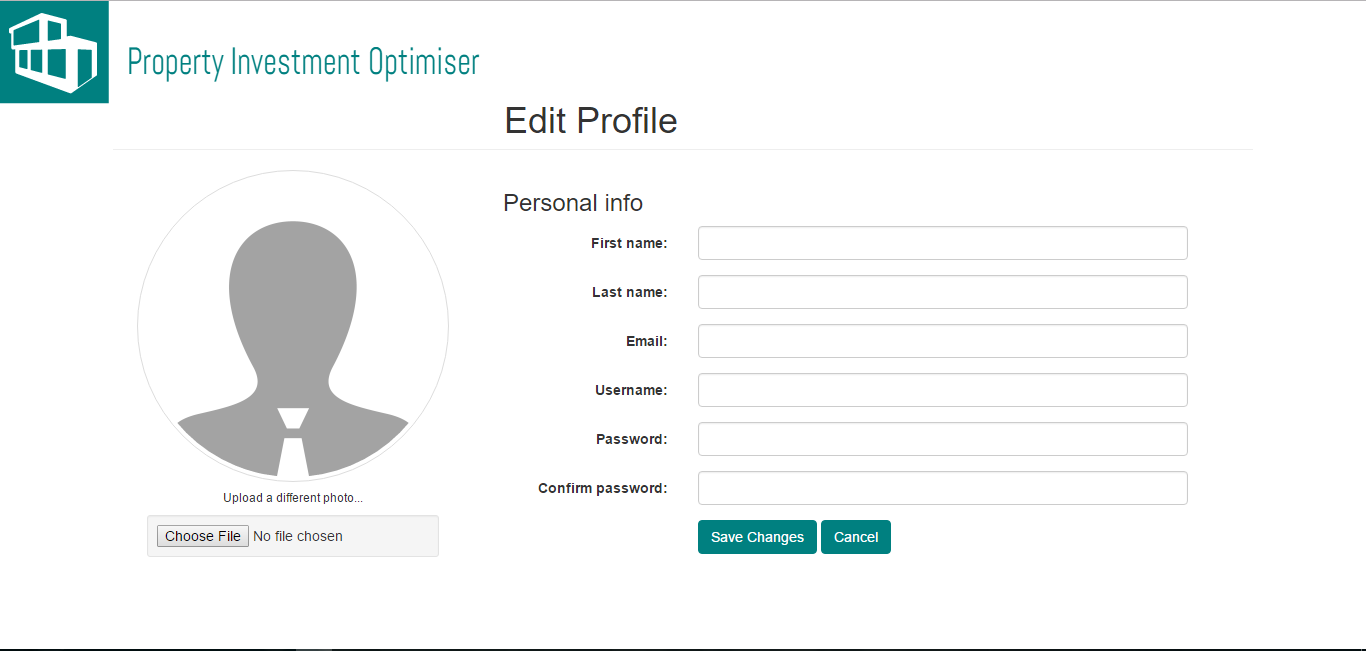
\includegraphics[width=0.9\linewidth, center]{./System/Profile.PNG}\\[0.4cm]  
		\caption{Profile}
This page will allow the user to change their login details and also to add extra details if they wish, like their full names and a profile picture.
\end{document}

